\section{Structure of the LHCb Detector}
The Large Hadron Collider beauty (LHCb) detector is a single-arm spectrometer possessing a forward angular coverage from
approximately 10 mrad to 300 (250) mrad in the bending (non-bending) plane \cite{https://doi.org/10.48550/arxiv.0910.1740}.
The structure of the detector is motivated by the fact that both the $b$ and the $\bar{b}$ hadrons are predominantly produced in the
same forward or backward cone. The components that enable the identification of particles, and aid the deduction of their properties include
the vertex locator system (VELO), the tracking system, comprising of a Trigger Tracker (a silicon microstrip detector, TT) located in front 
of the magnet, three tracking stations behind the magnet made up of silicon microstrips in the inner and outer parts (labelled IT and OT in Figure \ref{LHCbDetector} respectively),
two Ring Imaging Cherenkov counters (labelled RICH1 and RICH2 respectively), as well as a calorimeter system, comprising of a Scintillating Pad Detector and Preshower
(SPD/PS) and electromagnetic and hadronic calorimeters (ECAL and HCAL respectively) \cite{https://doi.org/10.48550/arxiv.0910.1740}. The layout of the LHCb spectrometer including the relative positions of the components described above, is illustrated in Figure \ref{LHCbDetector} below.\\
\\
Of the abovementioned components, the dipole magnet, VELO, ECAL, and the RICH detectors play a significant role
in the analysis of the decay described in Section \ref{DecayProcess}. The structure of these components of the
detector is further elaborated on in the sections that follow.
\begin{figure}[H]
    \centering
    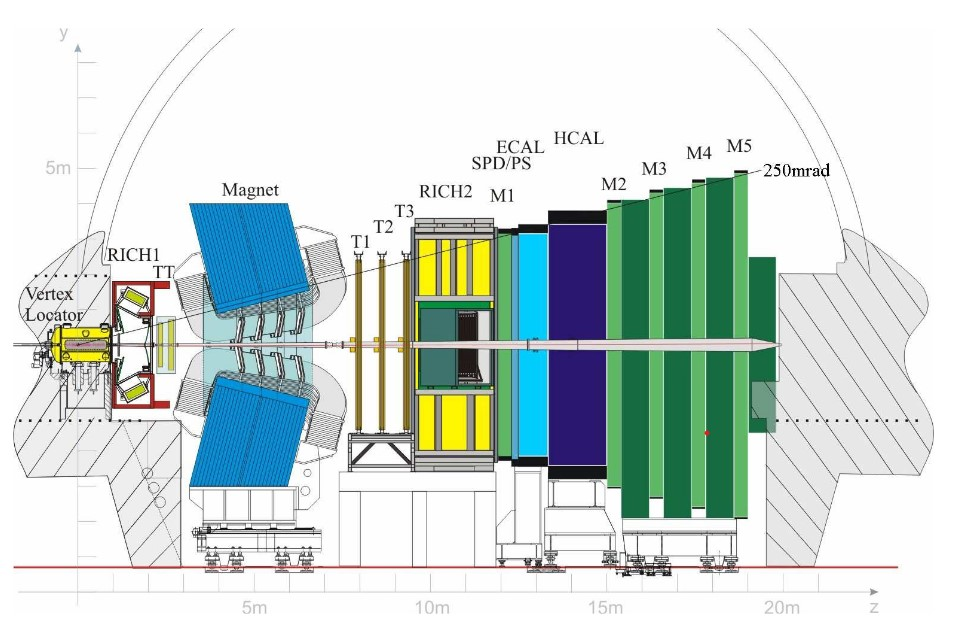
\includegraphics[scale = 0.45]{LHCbDetector.jpg}
    \caption{Diagram of the LHCb detector illustrating its various components. The coordinate system is oriented such that the beam is directed along the $z$ axis, and the $y$ axis is oriented along the vertical. Figure sourced from \cite{AbellanBeteta:2020amj}}
    \label{LHCbDetector}
\end{figure}
\subsection{Vertex Locator (VELO)}\label{VELO}
The Vertex Locator (VELO) is a silicon-tracking detector in the spectrometer, positioned around the proton-proton interaction region of the LHCb experiment shown in Figure \ref{LHCbDetector} above. It is responsible for the high-precision reconstruction of the primary and secondary vertices, and impact parameters of particle decays. In addition to this, it is a key
contributor to the measurements of particle lifetimes \cite{Kopciewicz_2022}. It was designed to optimise the angular coverage, triggering, reconstruction efficiency, and decay time of the resulting particles \cite{Aaij_2014}. The measurements made by the VELO are a vital input to the second level trigger (L1) which enhances the $b$-quark decay content of the data.\\
\begin{figure}[H]
    \centering
    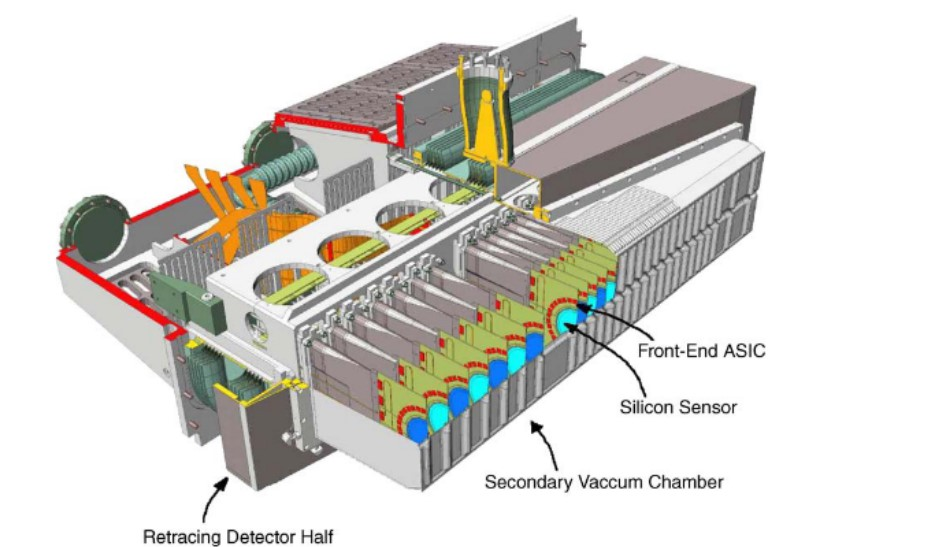
\includegraphics[scale=0.5]{VELOModule.jpg}
    \caption{Diagram representing one half of the VELO detector, illustrating the locations of the silicon sensors, and the Front-End ASICs that are crucial components of each module. Figure sourced from \cite{EKLUND200572}.}
    \label{VELOModule}
\end{figure}
The detector comprises of 21 silicon tracking stations that are placed orthognoally to the beam direction. These are placed around and downstream from the interaction point. Each of these stations consists of two detector modules that are mounted upon independent retracting detector supports, thereby enabling the retraction of the two detector halves during the set-up of the colliding beams \cite{EKLUND200572}. The double-sided detector modules contain two silicon sensors with different microstrip geometry, with one measuring the
radial distance from the beam axis (known as the R-sensor), and the other measuring an approximate azimuthal angle, $\phi$ (known as the $\phi$ sensor) \cite{Kopciewicz_2022}. The signals from the sensors are directed out via a second metal layer to an analogue front-end ASIC. The sensors and ASICs are mounted atop a TPG (Thermalised Pyrolytic Graphite) and carbon-fibre sandwich \cite{EKLUND200572}. The structure of one half of this sub-detector, including the locations of the abovementioned components is represented in Figure \ref{VELOModule} above. Refs \cite{Aaij_2014}, \cite{EKLUND200572}, and \cite{Kopciewicz_2022} provide a more detailed overview of the various components of the VELO. In addition to this, Ref \cite{Aaij_2014} presents a comprehensive account on the performance of this subdetector.

\subsection{Ring Imaging Cherenkov (RICH) Detectors}
The Ring Imaging Cherenkov (RICH) system at the LHCb consists of two detectors, namely RICH1 and RICH2, and is responsible for the identification of charged hadrons (such as $\pi, K$ and $p$). RICH1 is placed as close as possible to the interaction region, and is located immediately downstream of the VELO, described in Section \ref{VELO} above. This detector is intended to cover the low and intermediate momentum region (ranging from 2 to 40 GeV/c) over the full spectrometer angular acceptance of 25-300 mrad \cite{Adinolfi_2013}. RICH2, on the other hand, is placed downstream of the magnet, as it is intended to
identify particles possessing higher momenta (i.e. between 15-100 GeV/c) over the angular range 15-120 mrad, which are less affected by the magnetic field \cite{Adinolfi_2013}.\\
\\
RICH1 contains aerogel and two fluorobutane (C$_{4}$F$_{10}$) gas radiators which provide Particle Identification (PID) for positive kaons above 2 GeV/c and $\pi$-$K$ separation of up to 10 GeV/c.  within the acceptance. The detector consists of an optical system possessing spherical mirrors located in the LHCb acceptance that are traversed by charged particles and photons. The structure and materials used to construct these mirrors are elaborated upon in \cite{Antunes-Nobrega:630827}. The Cherenkov light emitted by particles as they traverse the detector is focused onto photon detector planes by these spherical mirrors, which are tilted, as well as secondary plane mirrors \cite{Antunes-Nobrega:630827}.Figure 
\ref{RICH1Layout} below illustrates the layout of the RICH1 detector, with the $z$ axis oriented to run horizontally. 
Further details on the structure and performance of RICH1 can be obtained in \cite{Adinolfi_2013} and \cite{Antunes-Nobrega:630827}. 
\begin{figure}[H]
    \centering
    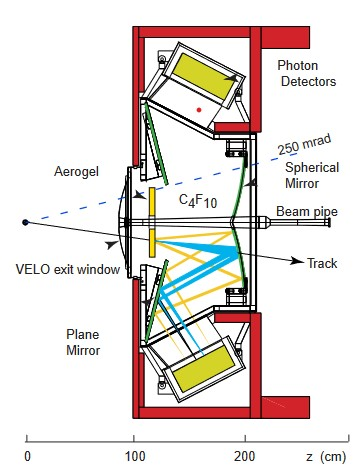
\includegraphics[scale=0.8]{RICH1Layout.jpg}
    \caption{Layout of the vertical RICH 1 detector, depicting the spherical and the secondary plane mirrors, as well as the region containing the gas radiators. The $z$-axis runs horizontally in this figure, and has units of cm. Figure sourced from \cite{Antunes-Nobrega:630827}}
    \label{RICH1Layout}
\end{figure}
The optical arrangement of the RICH2 detector is symmetric about the vertical plane. Much like RICH1, the detector possesses two sets of spherical and plane mirrors that focus Cherenkov radiationonto two photon detector arrays. CF$_{4}$ is used as the radiator material \cite{Harnew:2008zz}. Figure \ref{RICH2Layout} represents a schematic of the RICH2 detector.
\begin{figure}[H]
    \centering
    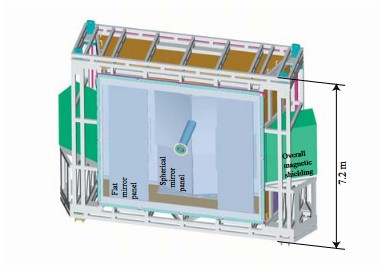
\includegraphics[scale = 1.2]{RICH2Layout.jpg}
    \caption{Schematic diagram of the RICH 2 detector, depicting the overall magnetic shielding (in green), and the flat and spherical mirror panels, labelled as such. Figure sourced from \cite{Harnew:2008zz}.}
    \label{RICH2Layout}
\end{figure}
\subsection{Magnet} 
The LHCb employs a warm dipole magnet (i.e. one that does not require cryogenic cooling) in order to measure the momenta of charged particles that traverse the detector. This measurement encompasses the forward acceptance of $\pm$ 250 mrad vertically and of $\pm$ 300 mrad horizontally \cite{Amato:424338}.
The magnet consists of saddle-shaped coils contained within a window-frame yoke with sloping poles, in alignment with the detector acceptance requirements. The magnet yoke possesses a symmetric structure, with two upright parts, each composed of laminated low carbon steel of thickness
100 mm, and weighing approximately 25 tons. The total weight of the yoke is approximately 1500 tons, and that of the two coils is 54 tons \cite{1018421}. These coils are placed mirror-symmetrically opposite each other within the magnet yoke, with each coil consisting of fifteen 'pancakes' arranged in five triplets.
Figure \ref{Magnet_image} below depicts the layout of the magnet, including the aforementioned components and the relative scale of the structure.
\begin{figure}[H]
    \centering
    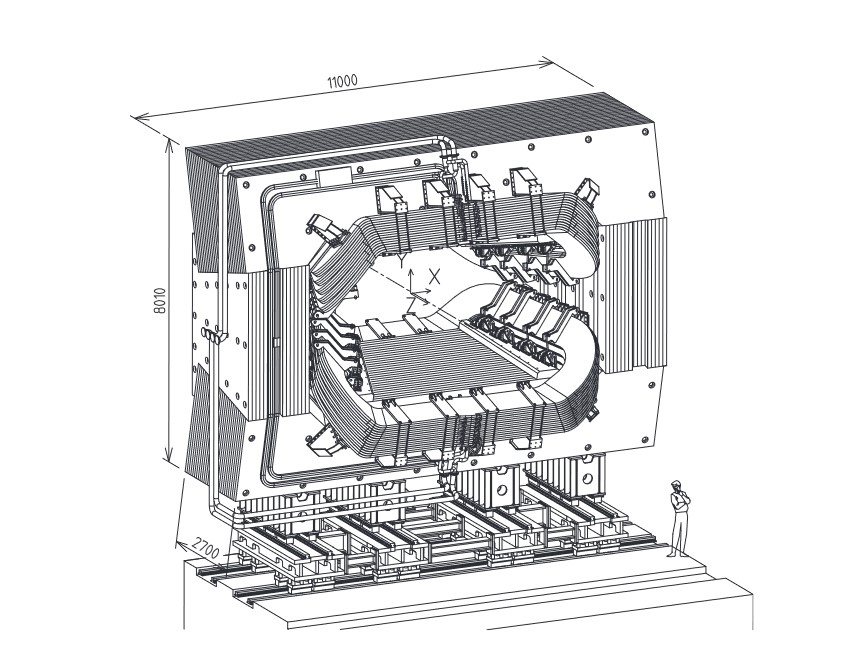
\includegraphics[scale=0.6]{Magnet_image.jpg}
    \caption{A perspective view of the LHCb dipole magnet with its current and water connections. The orientation of the coordinate system is also indicated on the diagram, where the units are measured in mm \cite{1018421}. The key components of the magnet described above, such as the yoke and the coils, are also visible. Figure sourced from \cite{1018421}.}
    \label{Magnet_image}
\end{figure}
The magnet is operated via the Magnet Control System, which regulates the power supply and monitors parameters such as temperatures, voltages, and mechanical movements. The safe operation of the magnet is monitored by a second, independent system known as the Magnet Safety System (MSS) \cite{1324843}. This system implements a discharge of the magnet if critical parameters stray outside of the operating range.
Further information on the structure and performance of this magnet can be obtained in Refs \cite{Amato:424338}, \cite{1018421}, and \cite{1324843}.

\subsection{Electromagnetic Calorimeter (ECAL)}
The ECAL aims to provide the precision measurement of photons in order to enable the reconstruction of $B$-decay modes containing either a photon or $\pi^{0}$ \cite{GOLUTVIN2003258}.
The calorimeter is constructed in a "shashlik" structure, comprising of three segmented sections, each comprising modules of an identical square size of 121.2 mm, but with varying numbers of
readout cells. This 'shashlik' structure had been chosen so as to enhance the energy resolution, response time, and the reliability of the calorimeter in an environment that is prone to radiation, in a cost effective manner \cite{Amato:494264}. Each module (depicted in Figure \ref{ECALModule} below) is comprised of alternating layers of a synthetic material made from polyethelene fibers known as Tyvek, a scintillator tile of thickness 4 mm, and a lead absorber plate of thickness 2 mm.
The system possesses a total of 67 scintillator and 66 absorber layers, combining to a resultant module depth of approximately 25 radiation lengths \cite{AbellanBeteta:2020amj}. The scintillation light is re-emitted and transported along fibres that penetrate the entire
module, and is then read out with a photomultiplier tube \cite{AbellanBeteta:2020amj}.

The energy resolution, $\frac{\sigma_{E}}{E}$, (i.e.the accuracy of the detector in determining the energy of the incoming radiation) of the outer module of the ECAL, which consists of one cell (depicted in Figures \ref{ECALModule} and \ref{ECALStructure} respectively) has been measured to be \cite{GOLUTVIN2003258}:
\begin{equation}
    \frac{\sigma_{E}}{E} = \frac{9.4\%}{\sqrt{E}}\oplus 0.8\%
\end{equation}
The ECAL is a key component of the search for ALPs at the LHCb experiment, since it measures the transverse energy $E_{T}$ of the photons in the decay channel of interest (see Section \ref{DecayChannel}), is a vital measurement for this analysis. Further details on the structure and performance of the ECAL can be obtained in Refs \cite{AbellanBeteta:2020amj}, \cite{Amato:494264}, and \cite{GOLUTVIN2003258}.
\begin{figure}[H]
    \begin{subfigure}{0.4\textwidth}
    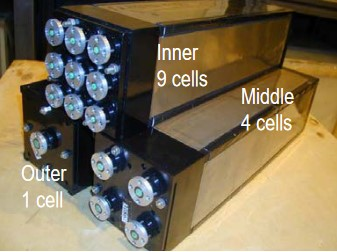
\includegraphics[scale = 0.8]{ECALModule.jpg}
    \caption{The inner, middle, and outer modules of the ECAL, consisting of 9, 4 and one cells respectively. Figure sourced from \cite{CERNLHCBECAL}}
    \label{ECALModule}
    \end{subfigure}
    \hfill
    \begin{subfigure}{0.5\textwidth}
        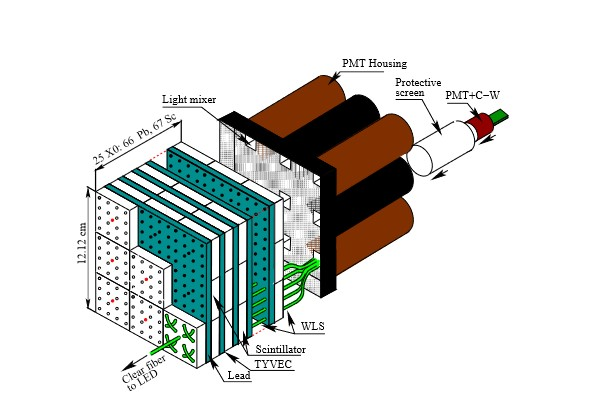
\includegraphics[scale = 0.7]{ECALStructure.jpg}
        \caption{Schematic diagram of an ECAL module, outlining its composition as well as the 'shashlik' structure made up of segmented sections of suitable materials. Figure sourced from \cite{AbellanBeteta:2020amj}.}
        \label{ECALStructure}
    \end{subfigure}
    \hfill
\end{figure}
\section{Data Analysis at the LHCb}
The Large Hadron Collider provides proton-proton collisions to the LHCb approximately 40 million times per second, thereby generating a significant amount of data \cite{LHCbSK}. In order to retain the data from events that are deemed to be of interest for analyses, the plethora of data must be filtered efficiently, and the algorithms
implemented must be sufficiently intricate, so as to be able to manage the complexity of the data being processed. The LHCb experiment implements a data flow which enables the aforementioned objectives to be addressed \cite{LHCbSK}. The flow of data through the LHCb system is further detailed in the sections that follow.
\subsection{The LHCb Data Flow}\label{LHCbDataFlow}
The collision events recorded by the LHCb detector proceed through various steps, each of which is controlled by an application that processes the data in a way that maximises the efficiency of data acquisition and also enhances the quality of the obtained. The data from the detector is first filtered through hardware and software components, known as the L0 trigger, and the high level trigger (HLT) respectively. Following this, the data is
reconstructed to transform the detector into objects such as tracks and clusters, which are stored in an output file in a 'DST' format. Data from this files is further filtered through a set of selections known as the stripping, the output of which is produced in either a DST or a '$\mu$DST' (micro-DST) format \cite{LHCbSK}.\\
\\
A substantial amount of Monte Carlo (MC) simulated data is also generated in parallel to the detector data as part of the data flow. This is processed in a very similar manner to the detector data outlined above \cite{LHCbSK}. Figure \ref{LHCbData} illustrates the abovementioned stages of the data flow and processing. The framework implemented to generate and process the simulated events described above, along with its constituent components that are highly relevant to the analysis of the decay of interest are further elaborated upon in the subsequent sections.
\begin{figure}[H]
    \centering
    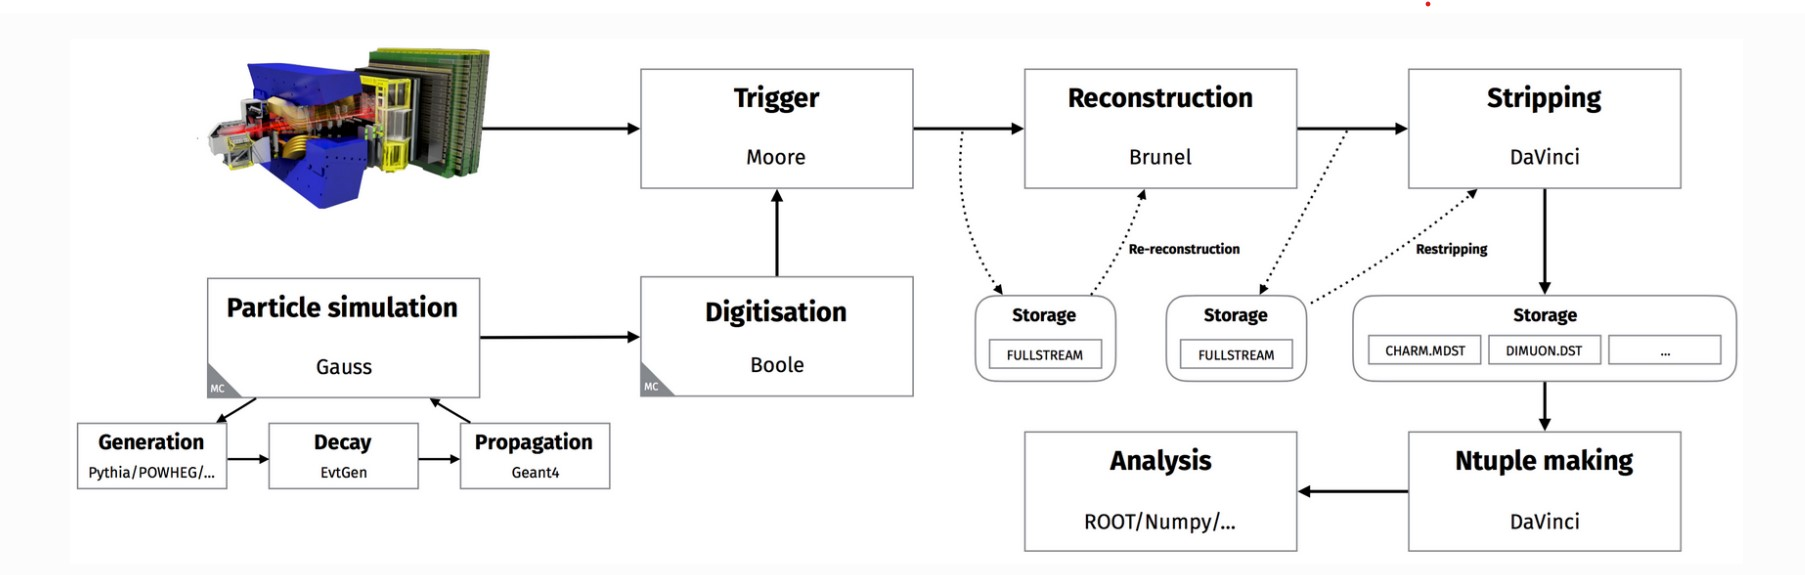
\includegraphics[scale = 0.4]{LHCbDataFlow.jpg}
    \caption{The LHCb Data Flow, outlining the various stages through which the data from the detector is processed, as well as the software applications responsible for the management of each stage. Figure sourced from \cite{LHCbSK}.}
    \label{LHCbData}
\end{figure}
\subsection{The LHCb Simulation Framework}
The MC simulated data that is processed in parallel to the detector data flows through a similar pipeline to its counterpart, with necessary steps in place to mimic the proton-proton collisions and the detector response. The former, and the subsequent hadronisation and decay of the resultant particles 
are controlled by the Gauss application, which is responsible for calling the various compatible Monte Carlo generators such as Pythia and POWHEG, as well as to control applications such as EvtGen and Geant4, which describe the decays of simulated particles and simulate their traversal through and interaction with
the detector \cite{LHCbSK}. On the other hand, the latter entails the transformation of the simulated hits made in the virtual detector into signals that mimic the real detector. This process is regulated by the Boole application, whose output is designed to closely match that of the real detector, such that the simulated data produced can be 
processed via the process described in Section \ref{LHCbDataFlow} above. The structure of the applications that are responsible for the simulation of the proton-proton collisions (such as Gauss, EvtGen, and Geant4) are described in the following sections, as these are fundamental for performing preliminary studies to determine the viability of the search for ALPs at the
LHCb.
\subsubsection{Gauss}
Gauss is a component of the simulation that intends to mimic the working of the spectrometer to enable the understanding of the experimental conditions and its performance \cite{Tlustos:913827}.
It comprises of two independent phases that are integrated and are typically run as a single job, but can be run separately if necessary. The first phase consists of the event generation
of proton-proton collisions and the decaying of the B mesons into channels of interest. This tool is interfaced to Pythia for the event production, and to a specialised decay package known as
EvtGen (see Section \ref{EvtGen} below). This phase also allows for the interfacing of other event generator engines if necessary. The particles produced are stored in the HepMC \cite{BUCKLEY2021107310} generic format that can be made persistent if the 
phase is run independently (i.e. in \textit{stand-alone} mode).\\
\\
The second phase consists of the tracking of the particles produced in the proton-proton interactions within the detector \cite{Belyaev_2011}. The physics processes undergone by the particles as they traverse the experimental setup are
regulated by the Geant4 toolkit (see Section \ref{Geant4} below), which interacts with Gauss using a host of interfaces and converters which enable the conversion of the LHCb detector geometry into the Geant4 geometry. In addition to this, it converts the output of the first phase of Gauss described above, to the Geant4 input format.\\
\\
Figure \ref{GaussSoftwareStructure} is a visual representation of the structure of the Gauss software that has been described above, while Figure \ref{GaussDependenices} depicts the various dependencies upon which the software has been built. These are further elaborated upon in the sections that follow. Further information on the architecture of the
Gauss software can also be obtained in \cite{Belyaev_2011} and \cite{Tlustos:913827}.
\begin{figure}[H]
    \begin{subfigure}{0.5\textwidth}
    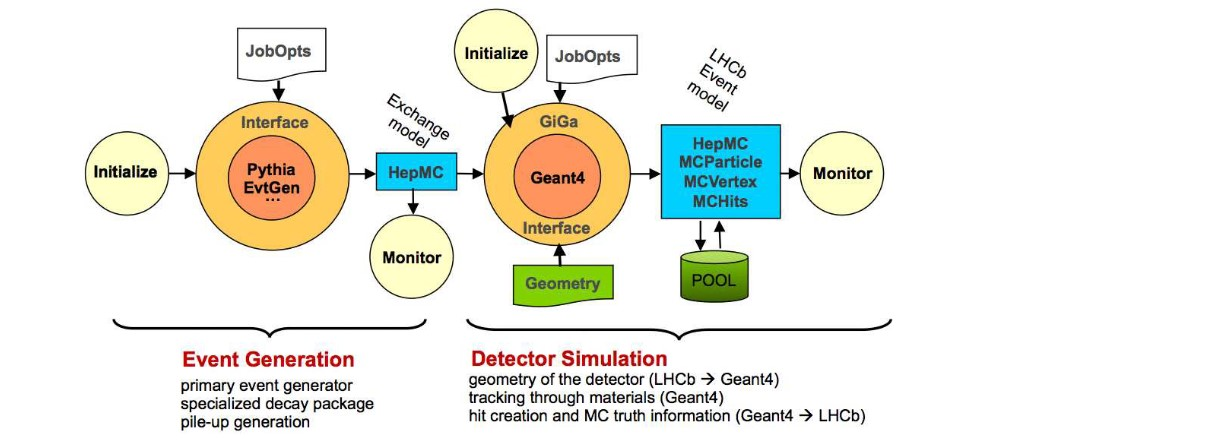
\includegraphics[scale = 0.5]{GaussSoftwareStructure.jpg}
    \caption{Visual representation of the structure of the Gauss software, depicting the Event Generation, and Detector Simulation phases, as well as the software dependencies necessary for data to be processed through these phases. Figure sourced from \cite{Belyaev_2011}}
    \label{GaussSoftwareStructure}
    \end{subfigure}
    \hfill
    \begin{subfigure}{0.4\textwidth}
        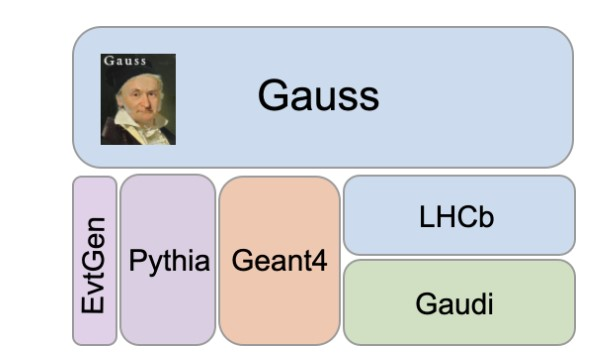
\includegraphics[scale = 0.55]{GaussDependenices.jpg}
        \caption{Representation of the underlying dependencies upon the Gauss simulation software, namely EvtGen, Pythia, EvtGen and the Gaudi franework, all of which are described in the sections that follow. Figure sourced from \cite{Tlustos:913827}}
        \label{GaussDependenices}
    \end{subfigure}
    \hfill
\end{figure}
\subsubsection{EvtGen}\label{EvtGen}
The EvtGen package is an event generator that is designed for the simulation of the physics of $B$-decays. The package provides a framework to handle complex sequential and CP violating decays. The simulation of these decays proceeds
using decay amplitudes, rather than probabilities. The amplitude for each node in a decay is used to simulate the entire decay chain, including all angular and time dependent correlations \cite{LANGE2001152}. The implementation of each decay amplitude is independent
of how the parent particle was produced, or how the daughter particles are to decay. The package implements an algorithmm that simulates correlations given individual decay amplitudes, which involves summing over the spin degrees of freedom of the daughters of the B-meson, to perform event selection. A more
detailed overview of this procedure can be obtained in \cite{LANGE2001152}.
\subsubsection{Pythia}
The PYTHIA program is a standard tool for the generation of high-energy collisions \cite{SJOSTRAND2015159}. It constitutes a coherent set of
physics models for the evolution from a few-body hard process to complex multihadronic final states, and contains numerous libraries of 
hard processes and models for initial and final state parton showers, multiple parton-parton interactions, beam remnants and particle decays. It 
also possesses a set of utilities and interfaces to external programs. The present version of the tool, PYTHIA 8, represents a complete rewrite in the C++ programming language, thereby contrasting
with its predecessors that were implemented in Fortran. The program presently only works with hadron-hadron and lepton-lepton collisions \cite{SJOSTRAND2015159}.\\
\\
Internally, the structure of Pythia can be divided into three main parts, namely the process level, the parton level, and the hadron level \cite{Bierlich:2022pfr}. The process level represents the hard-scattering processes, including the
production of short-lived resonances. The parton level accounts for initial and final-state radiation, by providing a multitude of shower models. At the completion of this stage of the event generation process, the user obtains a realistic
partonic structure, including jets, and the description of the underlying event, following which the hadron level becomes responsible for accounting for the effects of QCD confinement of partons into colour-singlet systems. In addition to this, the hadron level
also accountable for processes such as the decay of unstable hadrons and hadron rescattering. The output of this level is an event that is akin to one that can be observed in a detector. Details regarding each of the three levels described above, including the algorithms employed to generate
events can be obtained in \cite{Bierlich:2022pfr}.
\subsubsection{Geant4}\label{Geant4}
The Geant4 toolkit had been developed as the basis for the simulation framework, and as such, it is intended to have well-defined interfaces to other components, as well as to provide parts that can be used by these components. 
There exist seven key domains of the simulation of the traversal of particles through matter, namely \cite{GEANT4:2002zbu}:
\begin{itemize}
    \item Geometry and materials
    \item Particle interactions in matter
    \item Tracking management
    \item Digitisation and hit management
    \item Visualisation and visualisation framework
    \item User interface
\end{itemize}
Each of the domains described above are represented by class categories with coherent interfaces, and a corresponding working group with a well-defined responsibilities. The toolkit offers the user the ability to construct a geometric model 
with numerous components of varying shapes and materials. Furthermore, the user is able to define "sensitive" elements that enable the logging of information that is necessary to simulate detector responses.\\
\\
Geant4 also provides an extensive list of physics processes to model the behaviour of particles, enabling the user to choose between, add to, and modify a variety of implementations and approaches that are provided \cite{GEANT4:2002zbu}. In addition to this, the user is able to visualise the geometry
and tracks with a multitude of graphics systems and a user interface, which can be implemented over other systems of the user's choice. The structure of the toolkit can be described as a modular and hierarchical in nature, with dependencies forming links between the different sub-domains,
as illustrated in Figure \ref{Geant4Structure} below. Further detail on the nature of the sub-domains and dependencies depicted in this figure can be obtained in \cite{GEANT4:2002zbu}.
\begin{figure}[H]
    \centering
    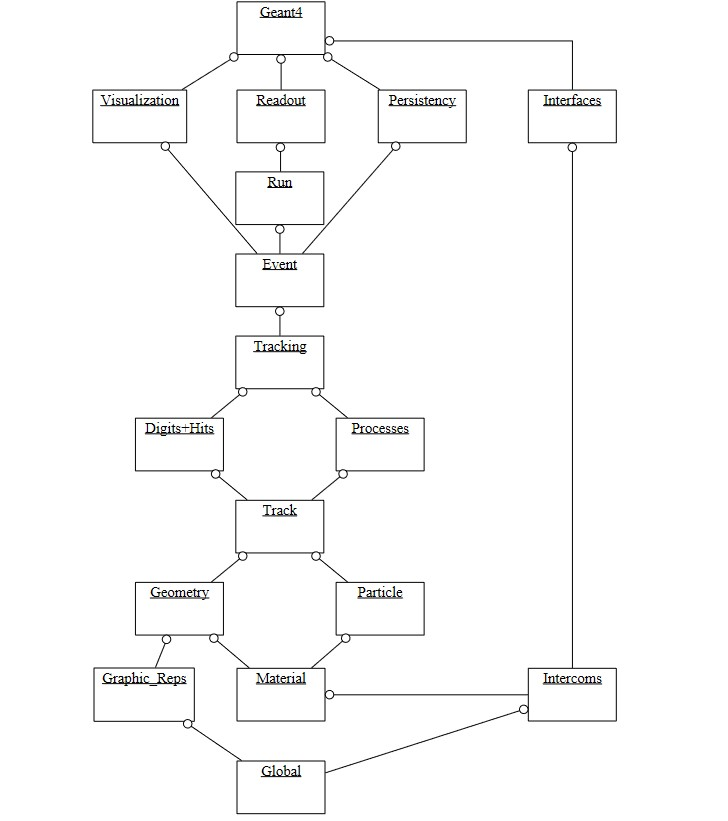
\includegraphics[scale=0.5]{Geant4Structure.jpg}
    \caption{Visual representation of the structure of the Geant4 software. The open circles on the joining lines signify a 'using' relationship, where the category at the end of the circle utilises the category that it is linked to. For instance, the Geometry category utilises the Material and Graphic\_Reps categories. Figure souced from \cite{GEANT4:2002zbu}.}
    \label{Geant4Structure}
\end{figure}
\subsubsection{Gaudi}
The Gaudi software has been developed with the intention of being able to build the large variety of applications necessary for high energy physics experiments, ranging from the simulation of events to the user analysis and the event display. Its design exploits object-oriented methodologies in order to address key criteria pertaining to the separation of data and algorithms, as well as that of persistent and transient data, among other aspects. It must be noted that all of the applicatios described in the previous
sections (i.e. Pythia, EvtGen, and Gauss) are built atop a Gaudi-based foundation, as depicted in Figure \ref{GaussDependenices}.\\
\\
The Gaudi architecture can broadly classified into three categories as follows \cite{BARRAND200145}:
\begin{itemize}
\item[-] \textbf{Algorithms and Application Manager:} Algorithms are a series of generic interfaces that are the fundamental components of applications that process event data. The application manager sits atop a hierarchy of algorithms, and is responsible for the instantiation and calling of these.
\item[-]\textbf{Transient Data Stores:} The data objects required by the algorithms are organised in various transient data stores, which store event data, which is valid only during the time it takes to process one event. Likewise, detector data, that generally has a lifetime of multiple events, is stored within the transient detector store. There also exists a data store for statistical data, which typically has the lifetime of a complete job, known as a transient histogram and n-tuple store. 
\item[-] \textbf{Services:} Services are a category of components which offer all the services necessary by algorithms (e.g. those for managing the various transient stores, or for managing the conversion between transient and persistent data). Services that facilitate visualisation and event selection also exist within the architecture.
\end{itemize}
Figure \ref{GaudiArchitecture} is a depiction of the Gaudi architecture described above.The key components (i.e. the algorithms, application manager, transient data stores, and services), as well as the relationship between these are indicated in this figure. Further detail on the nature of the components described in the diagram can be obtained in \cite{BARRAND200145} and \cite{Clemencic:2010zz}.
\begin{figure}[H]
    \centering 
    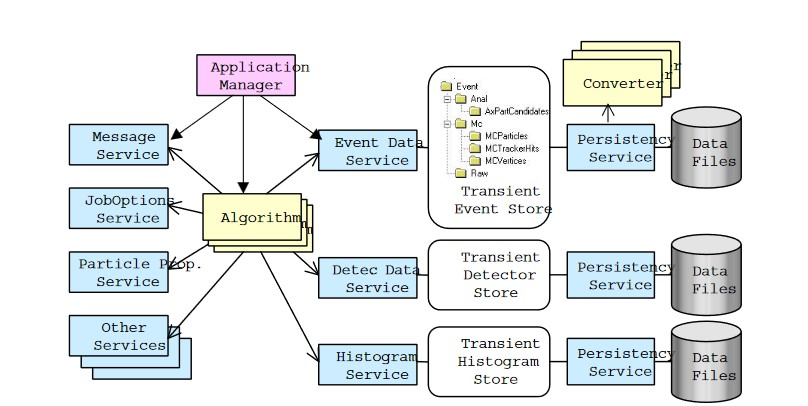
\includegraphics[scale=0.8]{GaudiArchitecture.jpg}
    \caption{A schematic diagram representing the architecture of the Gaudi software, including its constituent components such as the Algorithms and Application Manager, Transient Data Stores, and Services, as well as the interdependencies between these components. Figure sourced from \cite{GaudiArchitecture}.}
    \label{GaudiArchitecture}
\end{figure}



